\documentclass[a4paper,10pt]{article}
\usepackage[utf8x]{inputenc}
\usepackage{array}
\usepackage[pdftex]{graphicx}
\usepackage{hyperref}
\usepackage{listings}
\usepackage{enumitem}
\usepackage{color, colortbl}
\usepackage{longtable}
\usepackage{float}
\usepackage[compact]{titlesec}		% The 'compact' argument reduces spacing before/after headings

% Start ---- Fix for bug in issue 2.10.1 of titlesec package
\usepackage{etoolbox}

\makeatletter
\patchcmd{\ttlh@hang}{\parindent\z@}{\parindent\z@\leavevmode}{}{}
\patchcmd{\ttlh@hang}{\noindent}{}{}{}
\makeatother
% End ---- Fix for bug in issue 2.10.1 of titlesec package

\usepackage{verbatim}
\usepackage{fancyhdr}
\usepackage{parskip}
\usepackage{listings}
\usepackage{datatool}	% Management of external databases
\usepackage{pdflscape}	% Provides 'landscape mode' for selected pages
\usepackage{chngcntr}	% Management of figure and table numberings
\usepackage[ddmmyyyy]{datetime}

%------------------------------------------------------------------------------------------
% Directories holding image files:
% Figures from FW Profile Project and Figures from CORDET FW Project
%------------------------------------------------------------------------------------------
\graphicspath{ {../images/} }	

%---------------------------------------------
% Management of Figure and Table Numbering
%---------------------------------------------
\counterwithin{figure}{section}
\counterwithin{table}{section}

%---------------------------------------------
% Management of Captions
%---------------------------------------------
\usepackage[labelfont=bf]{caption}	% The caption label for tables and figures is bolded
\setlength{\abovecaptionskip}{0pt}	% Bring label close to figure or table
\renewcommand{\figurename}{Fig.}	% The caption label for figures is: "Fig."
\captionsetup[table]{singlelinecheck=off,justification=raggedright}	% Justify the table captions to the left

\pagestyle{fancy}

%---------------------------------------------
% Paragraph Layout
%---------------------------------------------
\setlength{\parindent}{0in}						% No indentation on first line of a new paragraph

%---------------------------------------------
% Definition of custom properties
%---------------------------------------------
\newcommand{\docIssue}{0.7.1}						% issue number
%\newcommand{\docDate}{30 December 2015}			% document date
\newcommand{\docRefNumber}{PP-SP-COR-0002}		% document reference number

%------------------------------------------------------------------------------------------
% Management of Headings
%------------------------------------------------------------------------------------------
% Define spacing to the left, before and after a subsection heading
%\titlespacing\subsubsection{8pt}{12pt plus 4pt minus 2pt}{-10pt plus 0pt minus 0pt}

% Introduce a page break before each section
\let\stdsection\section
\renewcommand\section{\newpage\stdsection}

%---------------------------------------------
% Headers and Footers
%---------------------------------------------
\renewcommand{\headrulewidth}{0.4pt}
\renewcommand{\footrulewidth}{0.4pt}

\lhead{\docRefNumber{}}
\chead{}
\rhead{Revision \docIssue{}}
\lfoot{\textcopyright2013 P\&P Software GmbH. All Rights Reserved.} 
\cfoot{\vspace{5mm}
{\color{red}\verbatiminput{../commercial/LicensedTo.txt}}}
\rfoot{\thepage}

%---------------------------------------------
% Management of lists
%---------------------------------------------
\setlist{nolistsep}								% No extra vertical space around a list		
\newenvironment{fw_itemize}						% Control spacing between items in a list
{\begin{itemize}
  \setlength{\itemsep}{1mm}
  \setlength{\parskip}{0pt}
  \setlength{\parsep}{0pt}}
{\end{itemize}}

\newenvironment{fw_enumerate}					% Control spacing between items in an enumeration
{\begin{enumerate}
  \setlength{\itemsep}{1mm}
  \setlength{\parskip}{0pt}
  \setlength{\parsep}{0pt}}
{\end{enumerate}}

%---------------------------------------------
% Paragraph Layout
%---------------------------------------------
\setlength{\parindent}{0in}						% No indentation on first line of a new paragraph

%---------------------------------------------
% Define Environment for Requirement Tables without Notes
% Par #1: Requirement Title
% Par #2: Requirement Verification Method
% Par #3: Requirement Text
% Par #4: Requirement Justification
% Par #5: Requirement Implementation
% Par #6: Requirement Verification
%---------------------------------------------
\newenvironment{fw_req}[6]
{\addtocounter{subsubsection}{1}
	\hspace{0.2cm}\textbf{CR-\arabic{section}.\arabic{subsection}.\arabic{subsubsection}/#2
	\hspace{0.8cm} #1}
	\vspace{-10pt}
\begin{longtable}{p{2.7cm}P{8.5cm}}
\hline
\textsc{Requirement} & #3 \\
\textsc{Justification} & #4 \\
\textsc{Implementation} & #5  \\ 
\textsc{Verification} & #6  \\
\hline
}
{\end{longtable}}

%---------------------------------------------
% Define Environment for Requirement Tables with Notes
% Par #1: Requirement Title
% Par #2: Requirement Verification Method
% Par #3: Requirement Text
% Par #4: Requirement Notes
% Par #5: Requirement Justification
% Par #6: Requirement Implementation
% Par #7: Requirement Verification
%---------------------------------------------
\newenvironment{fw_req_note}[7]
{\addtocounter{subsubsection}{1}
	\hspace{0.2cm}\textbf{FW-\arabic{section}.\arabic{subsection}.\arabic{subsubsection}/#2
	\hspace{0.8cm} #1}
	\vspace{-10pt}
\begin{longtable}{p{2.7cm}P{8.5cm}}
\hline
\textsc{Requirement} & #3 \\
\textsc{Note} & #4 \\
\textsc{Justification} & #5 \\
\textsc{Implementation} & #6  \\ 
\textsc{Verification} & #7  \\
\hline
}
{\end{longtable}}
	
%---------------------------------------------
% Define table layout 
%---------------------------------------------
\renewcommand{\arraystretch}{1.5}	% add vertical padding

\newcolumntype{P}[1]{>{%			% define column with paragraphs
  \parskip=0.5\baselineskip%
  \advance\parskip by 0pt plus 2pt
  \setlength{\parfillskip}{30pt plus 1fil}}p{#1}}


%---------------------------------------------
% Definition of colours
%---------------------------------------------
\definecolor{dkgreen}{rgb}{0,0.6,0}
\definecolor{gray}{rgb}{0.5,0.5,0.5}
\definecolor{mauve}{rgb}{0.58,0,0.82}
\definecolor{lightblue}{RGB}{128,179,255}
\definecolor{lbcolor}{rgb}{0.9,0.9,0.9}
\definecolor{light-gray}{gray}{0.85}
 
%---------------------------------------------
% Options for the code listing boxes
%---------------------------------------------
\lstset{ 
  language=C,                % the language of the code
  aboveskip=\bigskipamount,			% vertical space above listing box
  basicstyle=\footnotesize\ttfamily,    % use small size and mono-space font
  numbers=left,                   % where to put the line-numbers
  numberstyle=\tiny\color{gray},  % the style that is used for the line-numbers
  stepnumber=1,                   % the step between two line-numbers. If it's 1, each line 
                                  % will be numbered
  numbersep=5pt,                  % how far the line-numbers are from the code
  backgroundcolor=\color{lbcolor},      % choose the background color. You must add \usepackage{color}
  showspaces=false,               % show spaces adding particular underscores
  showstringspaces=false,         % underline spaces within strings
  showtabs=false,                 % show tabs within strings adding particular underscores
  frame=single,                   % adds a frame around the code
  rulecolor=\color{black},        % if not set, the frame-color may be changed on line-breaks within not-black text (e.g. commens (green here))
  tabsize=2,                      % sets default tabsize to 2 spaces
  captionpos=b,                   % sets the caption-position to bottom
  breaklines=true,                % sets automatic line breaking
  breakatwhitespace=false,        % sets if automatic breaks should only happen at whitespace
  title=\lstname,                   % show the filename of files included with \lstinputlisting;
                                  % also try caption instead of title
  keywordstyle=\color{blue},          % keyword style
  commentstyle=\color{dkgreen},       % comment style
  stringstyle=\color{mauve},         % string literal style
  escapeinside={\%*}{*)},            % if you want to add a comment within your code
  morekeywords={*,...}               % if you want to add more keywords to the set
}
 
%---------------------------------------------
% Title Page
%---------------------------------------------
\title{\textsc{The CORDET Framework} \\ \textsc{C2 Implementation} \\ \textsc{- USER REQUIREMENTS -}}
\author{Alessandro Pasetti \& Vaclav Cechticky}
\date{Created on: \today{}, at: \currenttime{}}

\begin{document}
\maketitle

\begin{center}
Revision \docIssue{} \\
\docRefNumber{}
\end{center}

\begin{center}
P\&P Software GmbH \\
High Tech Center 1 \\
8274 T\"{a}gerwilen \\
Switzerland \\
\vspace{2mm}
Web site: \url{www.pnp-software.com}\\
E-mail: \href{mailto:pnp-software@pnp-software.com}{\nolinkurl{pnp-software@pnp-software.com}} 
\end{center}


\begin{table}[ht]
\begin{center}
\begin{tabular}{p{11.7cm}}
\\
\hline
\end{tabular}
\end{center}
\end{table}
\begin{abstract}
This document defines, justifies, and verifies the User Requirements for the C2 Implementation of the CORDET Framework. The CORDET Framework is a software framework for service-oriented embedded applications. The CORDET Framework defines an application in terms of the services it provides to other applications and in terms of the services it uses from other applications.
\par
The CORDET Framework is implementation-independent. The C2 Implementation is a C-language implementation of the CORDET components. The main features of the C1 Implementation are: small memory footprint, small CPU demands, scalability, and high reliability.
\par 
The C2 Implementation is provided with a Qualification Data Package which can be used to support the certification of applications built using its components.
\end{abstract}
\begin{table}[ht]
\begin{center}
\begin{tabular}{p{11.7cm}}
\\
\hline
\end{tabular}
\end{center}
\end{table}

%---------------------------------------------
% Table of contents and list of figures and requirements
%---------------------------------------------
\newpage
\tableofcontents

\newpage
\listoffigures
\listoftables
%\lstlistoflistings

%---------------------------------------------
% Copyright notice
%---------------------------------------------

\newpage
\vspace*{\fill}
\begin{center}
No part of this publication may be reproduced, transmitted, transcribed, stored in any retrieval system, or translated into any language by any means without express prior written permission of P\&P Software GmbH.
\end{center}

\begin{center}
Copyright \textcopyright 2013 P\&P Software GmbH. All Rights Reserved. 
\end{center}
\vspace*{\fill}

%---------------------------------------------
% Adjust distance between paragraphs (this cannot be done earlier or it also affects the TOC)
%---------------------------------------------
\setlength{\parskip}{3mm}						% Set distance between paragraphs

%---------------------------------------------
% Start of Document Text
%---------------------------------------------

\newpage


\section{Introduction}
This document defines, justifies and verifies the user requirements for the \textit{C2 Implementation}. The C2 Implementation is a C-language implementation of the CORDET Framework. The CORDET Framework is a software framework for service-oriented distributed embedded applications. The CORDET Framework defines an application in terms of the services it provides to other applications and in terms of the services it uses from other applications.

A service is implemented by a set of commands through which an application is asked to perform certain activities and by a set of reports through which an application gives visibility over its internal state. The CORDET Framework defines the components to receive, send, distribute, and process commands and reports. The CORDET Framework is defined in \cite{ref:cordetfw}. 

\subsection{Intended Use of C1 Implementation}\label{sec:intendedUse}
Although the C2 Implementation can be used wherever there is a need to implement a system of distributed applications which exchange CORDET service requests, the high reliability of the implementation, the emphasis placed on formally specifying and verifying its expected behaviour, and the small demands on memory and processing resources mean that the C2 Implementation is especially well-suited for implementing mission-critical embedded applications within a service-oriented distributed architecture. 

Thus, the intended use of the C2 Implementation is to support the implementation of the CORDET service concept for mission-critical embedded applications.

\subsection{Requirement Definition}\label{sec:reqDef}
Requirements are defined in tables with the following format:

\hspace{0.2cm}\textbf{CR-'x'/'V' \hspace{0.9cm} $\langle$Requirement Title$\rangle$}
\vspace{-10pt}

\begin{longtable}{p{2.7cm}P{8.5cm}}
\hline
\textsc{Requirement} & $\langle$Formulation of requirement$\rangle$ \\
%\hline
\textsc{Note} & $\langle$Explicatory notes for requirement$\rangle$ \\
%\hline
\textsc{Justification} & $\langle$Justification of requirement$\rangle$ \\
%\hline
\textsc{Implementation} & $\langle$Dscription of how requirement is implemented$\rangle$ \\ 
%\hline
\textsc{Verification} & $\langle$Dscription of how requirement is verified$\rangle$ \\
\hline
\end{longtable}

Here, the suffix 'x' is a numerical identifier which uniquely identifies the requirement
within this document. The suffix 'V' identifies the verification method for the requirement according to the convention presented in section \ref{sec:reqVer}.

The explicatory notes are appended to the definition of the requirements where there is a need to clarify the terms which are used in their formulation.

In addition to their definition, this document also provides the following information for each requirement: a justification of the requirement; a description of how the requirement is implemented; and a description of how the requirement is verified. 

\subsubsection{Requirement Justification}
For each requirement, a \emph{justification} is provided which \emph{validates} the requirement. Requirements are justified with respect to the intended use of the C2 Implementation. The intended use of the C2 Implementation is to support the implementation of the CORDET service concept for mission-critical embedded applications (see section \ref{sec:intendedUse}).  Hence, a requirement is justified in proportion to its ability to further the adequacy of the C2 Implementation to support the implementation of the CORDET service concept in an environment where memory and processing resources are constrained and where reliability is of paramount importance. 

\subsubsection{Requirement Implementation}
For each requirement, the function or data structure or other code-level construct in the source code which implements it is identified.

\subsubsection{Requirement Verification}\label{sec:reqVer}
Verification information is provided for each requirement to demonstrate the correct implementation of the requirement. The following verification methods are possible:

\begin{fw_itemize}
\item Verification by Review ('R'): the requirement is verified by inspecting the code or its documentation.
\item Verification by Analysis ('A'): the requirement is verified by analysing the code, possibly with the help of a tool.
\item Verification by Test ('T'): the requirement is verified by one or more test cases in the Test Suite.
\end{fw_itemize}

One single verification method is defined for each requirement. 
This is identified as part of the requirement definition (see the description of the requirement format in section \ref{sec:reqDef}).

The Test Suite which is used for the verification by test is a complete application which demonstrates all aspects of the behaviour of the CORDET components. It consists of a sequence of Test Cases which are independent of each other. Each Test Case focuses on one particular functional aspect of the C2 Implementation. The Test Suite is distributed with the C2 Implementation. It is documented as part of the Doxygen documentation for the C2 Implementation and is described in the C2 Implementation User Manual (see reference \cite{ref:C2Implementation}).


%=============================================================================
% Introduce a page break before each sub-section
\let\stdsubsection\subsection
\renewcommand\subsection{\newpage\stdsubsection}
%=============================================================================


%=============================================================================
\section{Functional Requirements}\label{sec:fncReqs}
This section defines the functional requirements for the C2 Implementation. The functional requirements are those which define the functional behaviour of the components which implement the CORDET Framework.

%=============================================================================
\stdsubsection{CORDET Framework Requirements}\label{req:ImplCrReq}

The CORDET Framework is specified through a set of formal requirements defined in reference \cite{ref:cordetfw}. Four types of requirements are recognized in reference \cite{ref:cordetfw}: 

\begin{fw_itemize}
\item{} \textit{Standard Requirements} which define a desired feature of the framework. They are analogous in scope and format to the user requirements of an ordinary (non-framework) software application.
\item{} \textit{Adaptation Requirement} which define the points where the framework behaviour can be extended by the application developers (\textit{Adaptation Points}). In some cases, the definition of an adaptation point is accompanied by the definition of the default options offered by the framework for that adaptation point.  
\item{} \textit{Usage Constraint Requirements} which define the constraints on how the components offered by the framework may be used by application developers.
\item{} \textit{Property Requirements} which define behavioural properties which are guaranteed to hold on all applications which: (a) are instantiated from the framework by closing its adaptation points, and (b) comply with the framework's usage constraints.
\end{fw_itemize}

An implementation of the CORDET Framework should cover the first two types of requirements (the other two types of requirements are only relevant to application developers who wish to instantiate the framework to build a specific application). This section defines this coverage for the C2 Implementation.

%=============================================================================
\begin{fw_req}{CORDET Standard Requirements}{T}
{The C2 Implementation shall implement the standard requirements of the CORDET Framework of \cite{ref:cordetfw}.}
%-----------------------------------------------------------------------------
{The intended use of the C2 Implementation is to implement the CORDET Framework.}
%-----------------------------------------------------------------------------
{Appendix \ref{sec:implCrFwReq} shows how each standard requirement defined in reference \cite{ref:cordetfw} is implemented in the C2 Implementation.} 
%-----------------------------------------------------------------------------
{Appendix \ref{sec:implCrFwReq} shows how each standard requirement defined in reference \cite{ref:cordetfw} is verified in the C2 Implementation.} 
\end{fw_req}


%=============================================================================
\newpage
\begin{fw_req}{CORDET Adaptation Requirements}{R}
{The C2 Implementation shall implement the adaptation requirements of the CORDET Framework of reference \cite{ref:cordetfw}.}
%-----------------------------------------------------------------------------
{The intended use of the C2 Implementation is to implement the CORDET Framework.}
%-----------------------------------------------------------------------------
{The adaptation requirements of reference \cite{ref:cordetfw} define a number of adaptation points. Appendix \ref{sec:implCrFwAp} shows how each adaptation point of reference \cite{ref:cordetfw} is implemented in the C2 Implementation. } 
%-----------------------------------------------------------------------------
{See explanatory text at the beginning of appendix \ref{sec:implCrFwAp}. Note also that the Adaptation Requirements are verified by showing that a running application can be built by closing each Adaptation Point (or using the default value of an Adaptation Point). This is done in the Test Suite. The Test Suite exercises all framework functionalities (it has 100\% statement coverage) and therefore needs all Adaptation Points to be closed.}
\end{fw_req}

%=============================================================================
\subsection{C2 Adaptation Points}
%=============================================================================

\begin{fw_req}{C2 Adaptation Points}{R}
{The C2 Implementation shall support the adaptation points listed in table \ref{tab:implC2Ap}.}
%-----------------------------------------------------------------------------
{These adaptation points arise as a result of the design choices made for the C2 Implementation.}
%-----------------------------------------------------------------------------
{The last column in table \ref{tab:implC2Ap} describes how each adaptation points is implemented and what its default value (if any) is. } 
%-----------------------------------------------------------------------------
{See Implementation.}
\end{fw_req}


%=============================================================================
\begin{fw_req}{Default Values for Adaptation Points}{T}
{The C2 Implementation shall provide default values for all adaptation points (both those defined at CORDET Framework level and those defined at C2 Implementation level).}
%-----------------------------------------------------------------------------
{Provision of default values facilitates the definition of test cases and demonstrators.}
%-----------------------------------------------------------------------------
{The default values for the  column in table \ref{tab:implC2Ap} describes how each adaptation points is implemented and what its default value is. } 
%-----------------------------------------------------------------------------
{The default values for the C2 Implementation are those used for the Test Suite which constitutes a complete instantiation of the CORDET Framework and defined in appendix A of the reference \cite{ref:C2Implementation}.}
\end{fw_req}


%=============================================================================
\subsection{Component Instantiation}
%=============================================================================

\begin{fw_req}{Component Instantiation}{T}
{The C2 Implementation shall provide \textit{Factory Functions} to instantiate the following types of components: OutStream, OutFactory, OutManager, OutLoader, OutRegistry, InStream, InFactory, InManager, InLoader, and InRegistry.}
%-----------------------------------------------------------------------------
{The CORDET Framework distinguishes between components which are subject to \textit{early instantiation} and those which are subject to \textit{late instantiation} (see section 3.1 of reference \cite{ref:cordetfw}). The component types listed in this requirements are those which are subject to early instantiation. These are the components which must be instatiated during the application start-up.}
%-----------------------------------------------------------------------------
{The factory functions are the functions with names like: \texttt{CrFwXxxMake} where \texttt{Xxx} is the name of the component type. } 
%-----------------------------------------------------------------------------
{For each component type, a set of test cases is defined in: \texttt{CrFwXxxTestCases.h} where \texttt{Xxx} is the name of the component type. These test cases verify the factory functions.}
\end{fw_req}

%=============================================================================
\begin{fw_req}{Attribute Setting Order}{R}
{When a factory function configures a newly-created packet, it shall set its attributes in the following order: packet report/command flag (which determines whether the packet holds a report or a command), packet source (i.e. the host application), packet group, packet type, packet sub-type, packet discriminant, and then other attributes in an undefined order.}
%-----------------------------------------------------------------------------
{The framework provides one single interface for decoding and encoding packets in module \texttt{CrFwPckt}. This is obviously suitable for application developers who wish to use the same layout for all packets used by the application, irrespective of their type or of their destination or source or their other characteristics. If this is not possible, then the getter and setter functions of interface \texttt{CrFwPckt.h} must implement logic which makes their outcome dependent on the content of the packet itself. Thus, for instance, if different packet sources use different layouts, the getter functions will have to inspect the source of a packet before deciding how to decode the value of a packet's attribute. In the case of the setter functions, this approach requires that the order in which the packet attributes are set be specified so that the logic in the setter functions can rely on this ordering to decide how to set attribute values. }
%-----------------------------------------------------------------------------
{The only place in the CORDET Framework where newly-created packets are configured is the function to create a new OutComponent \texttt{CrFwOutFactoryMakeOutCmp}.} 
%-----------------------------------------------------------------------------
{Inspection of the implementation of function \texttt{CrFwOutFactoryMakeOutCmp} in module \texttt{CrFwOutFactory} shows that the requirement is fulfilled.}
\end{fw_req}


%=============================================================================
\begin{fw_req}{Irreversibility of Instantiation}{R}
{It shall not be possible to destroy an instance of the component types listed in the previous requirement.}
%-----------------------------------------------------------------------------
{The CORDET Framework specifies that components subject to early instantiation must be instantiated during the application start-up but it does not say whether they should be destroyed and re-created when the application is reset. In the interest of simplicity, the C2 Implementation bars dynamic destruction of these components.}
%-----------------------------------------------------------------------------
{The C2 Implementation does not define any \texttt{release} function through which the instances created by the Factory Functions may be destroyed. } 
%-----------------------------------------------------------------------------
{See implementation.}
\end{fw_req}





%=============================================================================
\subsection{Component Factories}
%=============================================================================

\begin{fw_req_note}{Component Pools in Factories}{R}
{The components factories of the C2 Implementation shall manage dynamic component creation through pools of pre-allocated component instances.}
%-----------------------------------------------------------------------------
{The component factories manage the dynamic allocation of components through a \texttt{make} and a \texttt{release} operation. The intention of this requirement is that these operations be implemented by creating a pool of pre-allocated components at initialization time and by then allocating and releasing component instances from this pool.}
%-----------------------------------------------------------------------------
{Use of a pre-allocated pool of component enchances static predictability of behaviour and this important for the target applications of the C2 Implementation.}
%-----------------------------------------------------------------------------
{There are only two factory components in the C2 Implementation: the OutFactory and the InFactory. The OutFactory defines array \texttt{outCmp} in \texttt{CrFwOutFactory.c} to hold the pre-allocated OutComponent instances. The InFactory defines arrays \texttt{inCmd} and \texttt{inRep} in \texttt{CrFwInFactory.c} to hold the pre-allocated InCommand and InReport instances. } 
%-----------------------------------------------------------------------------
{See Implementation.}
\end{fw_req_note}




%============================================================================
\begin{fw_req}{Dynamic Memory Allocation}{R}
{Dynamic memory allocation through calls to \texttt{malloc} shall be done exclusively as part of component initialization.}
%-----------------------------------------------------------------------------
{The component instantiation model of the CORDET Framework dictates that resource allocation be done as part of a component's Initialization Procedure (see section 3.2 of \cite{ref:cordetfw}.}
%-----------------------------------------------------------------------------
{Calls to \texttt{malloc} are used in the following functions: \texttt{CrFwInManagerInitAction}, \texttt{CrFwOutManagerInitAction} and \texttt{CrFwOutRegistryInitAction}. } 
%-----------------------------------------------------------------------------
{Functions \texttt{CrFwInManagerInitAction}, \texttt{CrFwOutManagerInitAction} and \texttt{CrFwOutRegistryInitAction} implement the initialization action of the InManager, OutManager and OutRegistry components and are therefore executed as part of these component initialization.}
\end{fw_req}


%============================================================================
\begin{fw_req}{Dynamic Memory Release}{R}
{If a component performs a \texttt{malloc} call as part of its initialization action, then it shall also perform a matching \texttt{free} call as part of its shutdown action.}
%-----------------------------------------------------------------------------
{The shutdown action is symmetric to the initialization action. This requirement therefore helps ensure that there are no memory leaks.}
%-----------------------------------------------------------------------------
{Calls to \texttt{free} are used in the following functions: \texttt{CrFwInManagerShutdown}, \texttt{CrFwOutManagerShutdown} and \texttt{CrFwOutRegistryShutdown}.   } 
%-----------------------------------------------------------------------------
{Functions \texttt{CrFwInManagerShutdown}, \texttt{CrFwOutManagerShutdown} and \texttt{CrFwOutRegistryShutdown} implement the shutdown operation of the InManager, OutManager and OutRegistry components which are the components which perform calls to \texttt{malloc} as part of their initialization (see previous requirement).}
\end{fw_req}









%======================================================================================
\section{Non-Functional Requirements}
%======================================================================================

This section defines the non-functional requirements of the C2 Implementation. Non-functional requirements impose overall constraints on the use, 
design, or implementation of the C2 Implementation.

%======================================================================================
\stdsubsection{Coding Requirements}\label{req:codingReqs}
%======================================================================================

\begin{fw_req}{Implementation Language}{R}
%-----------------------------------------------------------------------------
{The C2 Implementation shall be implemented in the ANSI C language.}
%-----------------------------------------------------------------------------
{The C Language is the standard language for embedded applications.}
%-----------------------------------------------------------------------------
{All the modules offered by the C2 Implementation are implemented in C and are compiled with the gcc compiler using the \texttt{-ansi -pedantic} option which enforces compliance with ANSI C.} 
%-----------------------------------------------------------------------------
{See implementation.}
%-----------------------------------------------------------------------------
\end{fw_req}


\begin{fw_req}{Compiler Warning}{T}
%-----------------------------------------------------------------------------
{The C2 Implementation shall not generate any warnings when compiled with the GCC compiler with all warnings enabled.}
%-----------------------------------------------------------------------------
{Warning may indicate weaknesses in the code or potential errors.}
%-----------------------------------------------------------------------------
{See verification.} 
%-----------------------------------------------------------------------------
{The C2 Implementation Acceptance Test Procedure (see reference \cite{ref:C2Implementation}) compiles all source files of the implementation using \texttt{gcc} with the option \texttt{-Wall}.}
%-----------------------------------------------------------------------------
\end{fw_req}


%======================================================================================
\subsection{Adaptation Mechanisms}\label{req:adaptationMechanisms}
%======================================================================================

\begin{fw_req_note}{Adaptation Mechanism}{R}
%-----------------------------------------------------------------------------
{The C2 Implementation shall exclusively support static adaptation mechanisms.}
%-----------------------------------------------------------------------------
{An adaptation mechanism is static if it only allows the adaptation to be performed at compile time. Thus, static adaptation forces application developers to decide how to close an adaptation point at compile time.}
%-----------------------------------------------------------------------------
{Restriction to static adaptation mechanisms enhances static predictability of behaviour which is important for mission-critical applications.}
%-----------------------------------------------------------------------------
{The adaptation mechanisms supported by the C2 Implementation are (see section 6 of reference \cite{ref:C2Implementation}):

\begin{fw_itemize}
\item Define Constant: a framework component uses a \texttt{\#DEFINE} constant whose value may be overridden by application developers.
\item Define Function: a framework component uses a function pointer and application developers must provide an implementation for the missing function (or, if available, may choose to use the default implementation provided at framework level)
\item Implement Interface: the framework defines an interface as a C header file and application developers must provide an implementation for it.
\item Define Type: a framework component uses a variables of a type defined as a \texttt{typedef} and application developers may override the default type definition.
\end{fw_itemize} } 
%-----------------------------------------------------------------------------
{The adaptation mechanisms listed above are compile-time adaptation mechanisms.}
%-----------------------------------------------------------------------------
\end{fw_req_note}


%======================================================================================
\subsection{Resource Requirements}\label{req:resourceReqs}
%======================================================================================

\begin{fw_req_note}{Code Memory Footprint}{T}
%-----------------------------------------------------------------------------
{The code memory footprint of the C2 Implementation shall be independent of the number of instances of framework components required by an application.}
%-----------------------------------------------------------------------------
{Ideally, it would be desirable to impose a requirement on the memory occupation 
of the C2 Implementation. This is not possible because memory occupation depends on the tool chain used to compile an application and on the target processor. This requirement aims to restrict memory occupation in a manner which is independent of the compilation tool chain and of the execution hardware.}
%-----------------------------------------------------------------------------
{Embedded applications are often memory-constrained.}
%-----------------------------------------------------------------------------
{See requirement verification.} 
%-----------------------------------------------------------------------------
{The C2 Implementation provides a set of factory functions and factory components to create instances of framework components. There is no code generation facility (neither explicit, nor implicit through the use of macros) which generates \emph{ad hoc} code for each component instance. Thus, the code base of the C2 Implementation is fixed and independent of the number of deployed component instances.}
%-----------------------------------------------------------------------------
\end{fw_req_note}


%======================================================================================
\subsection{Verification Requirements}\label{req:verificationReqs}
%======================================================================================

\begin{fw_req}{Test Coverage}{T}
%-----------------------------------------------------------------------------
{The C2 Implementation shall be provided with a Test Suite offering 100\% statement, branch and condition coverage.}
%-----------------------------------------------------------------------------
{The level of coverage provided by the requirement is that typically used in mission-critical applications.}
%-----------------------------------------------------------------------------
{The Test Suite is implemented in a set of Test Cases defined in \texttt{CrFwXxxTestCases.h} where \texttt{Xxx} is the name of a component type. The \texttt{main} program for the Test Suite is in \texttt{CrFwTestSuite.h}.} 
%-----------------------------------------------------------------------------
{The Acceptance Test Procedure of the C2 Implementation (see \cite{ref:C2Implementation}) uses the \texttt{gcov} tool to measure the statement and branch coverage of the Test Suite. Note that the C2 Implementation does not use any boolean expressions in the decision 
points of the code (e.g. in the \texttt{if} clauses). Decisions are always taken on the basis of the outcome of the evaluation of a single primitive Boolean condition. Hence, branch coverage implies condition coverage. In a few cases, the design may make full coverage impossible to achieve. The reason for the partial coverage is explained in comments in the code which are extracted and printed in the test report.}
%-----------------------------------------------------------------------------
\end{fw_req}





%======================================================================================
\subsection{Dependency Requirements}\label{req:dependencyReqs}
%======================================================================================

\begin{fw_req}{External Modules}{R}
%-----------------------------------------------------------------------------
{The C2 Implementation shall not require any external modules other than C's \texttt{stdlib} and \texttt{string} and the procedure and state machine modules of the C1 Implementation.}
%-----------------------------------------------------------------------------
{Minimization of dependencies on external libraries helps minimize the memory footprint of the application using the C2 Implementation and facilitates its qualification. The \texttt{stdlib} and \texttt{string} modules are likely to be used in any C application and hence they accepted. The C1 Implementation is provided with a qualification data package and its state machine and procedure modules have no external dependencies other than \texttt{stdlib} and \texttt{string}.}
%-----------------------------------------------------------------------------
{See verification.} 
%-----------------------------------------------------------------------------
{Inspection of the C2 Implementation files shows that no external modules other than \texttt{stdlib} and \texttt{string} and the state machine modules \texttt{FwSm*.h} and the procedure modules \texttt{FwPr*.h} of the C1 Implementation are used. The compilation and linking process for the Test Suite shows that no other libraries need be linked.}
%-----------------------------------------------------------------------------
\end{fw_req}


%=====================================================================================

\appendix
\section{CORDET Framework Standard Requirements}\label{sec:implCrFwReq}
The C2 Implementation implements the standard requirements of the CORDET Framework. 
Table \ref{tab:implCrFwReq} lists the standard requirements of the CORDET Framework as they are defined in reference \cite{ref:cordetfw} and, for each requirement, it describes how the requirement is implemented in the C2 Implementation and how the implementation is verified. The requirement identifier (first column in the table) is the same as used in reference \cite{ref:cordetfw}.

The requirements often refer to state machine or procedure diagrams. A complete list of the diagrams of the state machines and procedures which define the behaviour of the CORDET components can be found in section \ref{sec:smAndProcDiagrams}.

\DTLloaddb{dbCrFwReq}{../cordetfw/CordetFwReq.csv}	% Import table with CORDET FW Req

\begin{landscape}

\begin{longtable}{|>{\centering\arraybackslash}p{0.9cm}|>{\raggedright}p{4.9cm}|p{6.9cm}|p{6.9cm}|}
\caption{Implementation of CORDET Framework Requirements} \label{tab:implCrFwReq}\\
\hline
\rowcolor{light-gray}
\textbf{ID} & \textbf{Requirement Text} & \textbf{Requirement Implementation} & \textbf{Requirement Verification} \\
\hline\hline
\endfirsthead
\rowcolor{light-gray}
\textbf{ID} & \textbf{Requirement Text} & \textbf{Requirement Implementation} & \textbf{Requirement Verification} \\
\hline\hline
\endhead
\DTLforeach*[\DTLiseq{\type}{S}]{dbCrFwReq}{\cat=Category,\type=Type,\id=Id,\reqText=Text,\reqImpl=Implementation,\reqVer=Verification}
{\DTLiffirstrow{}{\\\hline}\cat-\id & \reqText & \reqImpl & \reqVer}\\\hline
\end{longtable}

\end{landscape}

%======================================================================================
\section{CORDET Framework Adaptation Points}\label{sec:implCrFwAp}
The C2 Implementation implements the adaptation points of the CORDET Framework.
Table \ref{tab:implCrFwAp} lists the adaptation points of the CORDET Framework as they are defined in reference \cite{ref:cordetfw}. The requirement identifier (first column in the table) is the same as used in reference \cite{ref:cordetfw}. 

For each adaptation point, the last column in the table either describes how the adaptation point is implemented in the C2 Implementation or it explains why it is not directly implemented. The latter is the case for the following kinds of adaptation points:

\begin{fw_itemize}
\item Adaptation points which are "closed at framework level" and which are therefore not present in the C2 Implementation. This is the case when component B is derived (through the extension mechanism of the FW Profile) from component A and component A has defined an adaptation point which is inherited by component B but which component B closes (i.e. the value of the adaptation point on component B is fixed and cannot be modified by users of the framework). Thus, for instance, the Execution Procedure is an adaptation point for the Base Component (BAS-6) but the framework components which are derived from the Base Component have a specific Execution Procedure which is not intended to be modified by application developers and therefore "close" the adaptation point BAS-6 defined on the Base Component.
\item Adaptation points which have been mapped to other adaptation points which are specific to the C2 Implementation. In these cases, the last column in the table identifies the C2 Implementation adaptation point (the full list of C2 Implementation Points is provided in appendix \ref{sec:implC2Ap}).
\item Adaptation points which are closed as a result of the design choices made by the C2 Implementation. This is, for instance, the case for the adaptation points for the OutStreamRegistry. In the C2 Implementation, this component has been merged with the OutStream component and hence its adaptation points have been merged with those of the OutStream.
\end{fw_itemize}

The definitions of the CORDET adaptation points often refer to state machine or procedure diagrams. A complete list of the diagrams of the state machines and procedures which define the behaviour of the CORDET components can be found in section \ref{sec:smAndProcDiagrams}.

\DTLloaddb{dbAP}{../cordetfw/CordetFwAP.csv}	% Import table adaptation points

\begin{landscape}

\begin{longtable}{|l|p{4.2cm}|p{5.0cm}|p{8.4cm}|}
\caption{CORDET Adaptation Points} \label{tab:implCrFwAp}\\
\hline
\rowcolor{light-gray}
\textbf{AP ID} & \textbf{Adaptation Point} & \textbf{Default Value} & \textbf{Implementation}\\ 
\hline\hline
\endfirsthead
\rowcolor{light-gray}
\textbf{AP ID} & \textbf{Adaptation Point} & \textbf{Default Value} & \textbf{Implementation}\\
\hline\hline
\endhead
\DTLforeach*[\not\DTLiseq{\cat}{0}]{dbAP}{\cat=Category,\id=Id,\dv=DefValue,\ap=AP,\impl=C2Impl}
{\DTLiffirstrow{}{\\\hline}\cat-\id & \ap & \dv & \impl}\\\hline
\end{longtable}

\end{landscape}

%======================================================================================
\section{C2 Adaptation Points}\label{sec:implC2Ap}
The C2 Implementation implements the adaptation points of the CORDET Framework.
Table \ref{tab:implCrFwAp} lists the adaptation points of the CORDET Framework as they are defined in reference \cite{ref:cordetfw} and, for each adaptation point, it describes how the adaptation point is implemented in the C2 Implementation. 

Besides the adaptation points defined by the CORDET Framework, the C2 Implementation also provides a number of additional adaptation points which arise as a result of the design choices made for the C2 Implementation. These adaptaton points are called \textit{C2 Adaptation Points} and are listed in table \ref{tab:implC2Ap}. The last column in the table shows how each adaptation point is implemented and which default value (if any) is offered for it by the C2 Implementation.

The definitions of the C2 adaptation points often refer to state machine or procedure diagrams. A complete list of the diagrams of the state machines and procedures which define the behaviour of the CORDET components can be found in section \ref{sec:smAndProcDiagrams}.

\begin{landscape}

\begin{longtable}{|l|p{5.2cm}|p{13.0cm}|}
\caption{C2 Adaptation Points} \label{tab:implC2Ap}\\
\hline
\rowcolor{light-gray}
\textbf{AP ID} & \textbf{Adaptation Point} & \textbf{Implementation}\\ 
\hline\hline
\endfirsthead
\rowcolor{light-gray}
\textbf{AP ID} & \textbf{Adaptation Point} & \textbf{Implementation}\\
\hline\hline
\endhead
\DTLforeach*[\not\DTLiseq{\cat}{0}]{dbAP}{\cat=C2Cat,\id=C2Id,\ap=AP,\impl=C2Impl}
{\DTLiffirstrow{}{\\\hline}\cat-\id & \ap & \impl}\\\hline
\end{longtable}

\end{landscape}


%======================================================================================
\section{CORDET Framework Behaviour}\label{sec:verCrFwBehaviour}
The C2 Implementation implements the behaviour of the CORDET Framework. The behaviour of the CORDET Framework is defined through a set of state machines and procedures (see \ref{sec:smAndProcDiagrams} for a full list of their diagrams). Thus, the C2 Implementation implements the behaviour of the CORDET Framework state machines and procedures. This section provides the verification evidence which demonstrates correct implementation of the CORDET Framework state machines and procedures.  


%--------------------------------------------------------------------------------------
\stdsubsection{Verification of State Machine Behaviour}
Correct implementation of the state machine behaviour is verified at the level of the C1 Implementation in reference \cite{ref:C1UserReq}. At the level of the C2 Implementation it is therefore only necessary to verify that the state machines are correctly configured. This is done by performing tests which:

\begin{fw_enumerate}
\item For every transition in the state machine, execute the state transition 
\item For every transition originating in a proper state which has a guard, attempt to execute the state transition with the guard evaluating to false
\item For every do action in the state machine, execute the state machine
\end{fw_enumerate}

Note that the first two bullets also verify execution of all entry, exit and transition actions in the state machine. Tables \ref{tab:verBaseSM} to \ref{tab:verInCmdSM} provide this verification evidence for each state machine defined in reference \cite{ref:cordetfw}. For each element in the previous list to be verified, the tables give the name of the test case in the Test Suite where that element is verified. Note that no attempt is made to list all test cases which verify a given element; rather the ojective is to identify one test case for each element to be verified. 

\begin{longtable}{|>{\raggedright}p{6.0cm}|P{5.0cm}|}
\caption{Verification of Base State Machine}
\label{tab:verBaseSM}\\
\hline
\rowcolor{gray}
\textbf{Element} & \textbf{Test Case} \\
\hline
\endfirsthead
\rowcolor{gray}
\textbf{Element} & \textbf{Test Case} \\
\hline
\endhead
Transition from Initial Pseudo-State to CREATED  & \texttt{CrFwBaseCmpTestCase1}\\
\hline
Transition from CREATED to CREATED  & \texttt{CrFwInStreamTestCase5}\\
\hline
Transition from CREATED to INITIALIZED  & \texttt{CrFwBaseCmpTestCase1}, \texttt{CrFwInStreamTestCase5}\\
\hline
Transition from INITIALIZED to INITIALIZED  & \texttt{CrFwInStreamTestCase5}\\
\hline
Transition from INITIALIZED to CONFIGURED  & \texttt{CrFwBaseCmpTestCase1}, \texttt{CrFwInStreamTestCase5}\\
\hline
Transition from CONFIGURED to CONFIGURED  & \texttt{CrFwInStreamTestCase4}\\
\hline
Transition from CONFIGURED to Final Pseudo-State  & \texttt{CrFwInStreamTestCase6}\\
\hline
Do Action in CONFIGURED & \texttt{CrFwInLoaderTestCase2} to \texttt{CrFwInLoaderTestCase11} verify that execution of InLoader component in state CONFIGURED triggers execution of its Execution Procedure \\
\hline
\end{longtable}

\begin{longtable}{|>{\raggedright}p{6.0cm}|P{5.0cm}|}
\caption{Verification of Application State Machine}
\label{tab:verAppSM}\\
\hline
\rowcolor{gray}
\textbf{Element} & \textbf{Test Case} \\
\hline
\endfirsthead
\rowcolor{gray}
\textbf{Element} & \textbf{Test Case} \\
\hline
\endhead
Transition from Initial Pseudo-State to START-UP  & \texttt{CrFwAppSmTestCase1}\\
\hline
Transition from START-UP to NORMAL with transition guard true  & \texttt{CrFwAppSmTestCase1}\\
\hline
Transition from START-UP to NORMAL with transition guard false  & \texttt{CrFwAppSmTestCase1}\\
\hline
Transition from NORMAL to RESET & \texttt{CrFwAppSmTestCase1}\\
\hline
Transition from RESET to NORMAL with transition guard true  & \texttt{CrFwAppSmTestCase1}\\
\hline
Transition from RESET to NORMAL with transition guard false  & \texttt{CrFwAppSmTestCase1}\\
\hline
Transition from NORMAL to SHUTDOWN & \texttt{CrFwAppSmTestCase1}\\
\hline
Transition from SHUTDOWN to Final-Pseudo State with transition guard true  & \texttt{CrFwAppSmTestCase1}\\
\hline
Transition from SHUTDOWN to Final-Pseudo State with transition guard false  & \texttt{CrFwAppSmTestCase1}\\
\end{longtable}

\begin{longtable}{|>{\raggedright}p{6.0cm}|P{5.0cm}|}
\caption{Verification of OutStream State Machine}
\label{tab:verOutStreamSM}\\
\hline
\rowcolor{gray}
\textbf{Element} & \textbf{Test Case} \\
\hline
\endfirsthead
\rowcolor{gray}
\textbf{Element} & \textbf{Test Case} \\
\hline
\endhead
Transition from Initial Pseudo-State to READY  & \texttt{CrFwOutStreamTestCase1}\\
\hline
Transition from READY to Choice Pseudo-State & \texttt{CrFwOutStreamTestCase1}\\
\hline
Transition from Choice Pseudo-State to BUFFERING & \texttt{CrFwOutStreamTestCase1}\\
\hline
Transition from BUFFERING to BUFFERING & \texttt{CrFwOutStreamTestCase1}\\
\hline
Transition from BUFFERING to Choice Pseudo-State & \texttt{CrFwOutStreamTestCase3}\\
\hline
Transition from Choice Pseudo-State to READY & \texttt{CrFwOutStreamTestCase3}\\
\hline
In Enqueue Action, Branch with PQ not full & \texttt{CrFwOutStreamTestCase1}\\
\hline
In Enqueue Action, Branch with PQ full & \texttt{CrFwOutStreamTestCase1}\\
\hline
In Send or Enqueue Action, Branch with Packet Not Originating in Application & \texttt{CrFwOutStreamTestCase6}\\
\hline
In Send or Enqueue Action, Branch with Middleware Accepting Packet & \texttt{CrFwOutStreamTestCase3}\\
\hline
In Send or Enqueue Action, Branch with Middleware Rejecting Packet & \texttt{CrFwOutStreamTestCase3}\\
\hline
In Send or Enqueue Action, Branch with Legal Group & \texttt{CrFwOutStreamTestCase3}\\
\hline
In Send or Enqueue Action, Branch with Illegal Group & \texttt{CrFwOutStreamTestCase7}\\
\hline
In Flush Packet Queue Action, Branch with Packet Originating in Application & \texttt{CrFwOutStreamTestCase3}\\
\hline
In Flush Packet Queue Action, Branch with Legal Packet Group & \texttt{CrFwOutStreamTestCase3}\\
\hline
In Flush Packet Queue Action, Branch with Packet Not Originating in Application & \texttt{CrFwOutStreamTestCase6}\\
\hline
In Flush Packet Queue Action, Branch with Middleware Accepting Packet & \texttt{CrFwOutStreamTestCase3}\\
\hline
In Flush Packet Queue Action, Branch with Middleware Rejecting Packet & \texttt{CrFwOutStreamTestCase3}\\
\hline
In Flush Packet Queue Action, Branch with Legal Group & \texttt{CrFwOutStreamTestCase3}\\
\hline
In Flush Packet Queue Action, Branch with Illegal Group & \texttt{CrFwOutStreamTestCase7}\\
\hline
\end{longtable}



\begin{longtable}{|>{\raggedright}p{6.0cm}|P{5.0cm}|}
\caption{Verification of InStream State Machine}
\label{tab:verInStreamSM}\\
\hline
\rowcolor{gray}
\textbf{Element} & \textbf{Test Case} \\
\hline
\endfirsthead
\rowcolor{gray}
\textbf{Element} & \textbf{Test Case} \\
\hline
\endhead
Transition from Initial Pseudo-State to WAITING  & \texttt{CrFwInStreamTestCase1}, \texttt{CrFwInStreamTestCase4}\\
\hline
Transition from Initial Pseudo-State to PCKT\_AVAIL  & \texttt{CrFwInStreamTestCase6}\\
\hline
Transition from PCKT\_AVAIL to PCKT\_AVAIL through Choice Pseudo-State  & \texttt{CrFwInStreamTestCase2}\\
\hline
Transition from WAITING to WAITING through Choice Pseudo-State  & \texttt{CrFwInStreamTestCase2}\\
\hline
Transition from PCKT\_AVAIL to PCKT\_AVAIL through Self-Transition  & \texttt{CrFwInStreamTestCase3}, \texttt{CrFwInStreamTestCase4}\\
\hline
Transition from PCKT\_AVAIL to WAITING  & \texttt{CrFwInStreamTestCase2}\\
\hline
Transition from WAITING to PCKT\_AVAIL  & \texttt{CrFwInStreamTestCase2}, \texttt{CrFwInStreamTestCase3}, \texttt{CrFwInStreamTestCase4}\\
\hline
\end{longtable}

\begin{longtable}{|>{\raggedright}p{6.0cm}|P{5.0cm}|}
\caption{Verification of OutComponent State Machine}
\label{tab:verOutComponentSM}\\
\hline
\rowcolor{gray}
\textbf{Element} & \textbf{Test Case} \\
\hline
\endfirsthead
\rowcolor{gray}
\textbf{Element} & \textbf{Test Case} \\
\hline
\endhead
Transition from Initial Pseudo-State to LOADED  & \texttt{CrFwOutCmpTestCase2} to \texttt{CrFwOutCmpTestCase6}\\
\hline
Transition from LOADED to ABORTED  & \texttt{CrFwOutCmpTestCase2}, \texttt{CrFwOutCmpTestCase6}\\
\hline
Transition from LOADED to PENDING  & \texttt{CrFwOutCmpTestCase3} to \texttt{CrFwOutCmpTestCase9}\\
\hline
Transition from PENDING to TERMINATED with guard true and a valid OutStream (i.e. transition is triggered by Repeat Check returning 'no repeat') & \texttt{CrFwOutCmpTestCase7}\\
\hline
Transition from PENDING to TERMINATED with guard true due to an invalid OutStream (i.e. transition is triggered by Send Packet Procedure having set \texttt{isRepeat} to 'no repeat') & \texttt{CrFwOutCmpTestCase8}\\
\hline
Transition from PENDING to TERMINATED with guard false & \texttt{CrFwOutCmpTestCase7}\\
\hline
Transition from PENDING to ABORTED with guard true & \texttt{CrFwOutCmpTestCase9}\\
\hline
Transition from PENDING to ABORTED with guard false & \texttt{CrFwOutCmpTestCase7}, \texttt{CrFwOutCmpTestCase8}\\
\hline
\end{longtable}

\begin{longtable}{|>{\raggedright}p{6.0cm}|P{5.0cm}|}
\caption{Verification of InCommand State Machine}
\label{tab:verInCmdSM}\\
\hline
\rowcolor{gray}
\textbf{Element} & \textbf{Test Case} \\
\hline
\endfirsthead
\rowcolor{gray}
\textbf{Element} & \textbf{Test Case} \\
\hline
\endhead
Transition from Initial Pseudo-State to ACCEPTED  & \texttt{CrFwOutCmpTestCase1} to \texttt{CrFwOutCmpTestCase3} and \texttt{CrFwOutCmpTestCase5} to \texttt{CrFwOutCmpTestCase11} \\
\hline
Transition from ACCEPTED to Choice Psedo-State with guard false & \texttt{CrFwOutCmpTestCase2}\\
\hline
Transition from ACCEPTED to ABORTED & \texttt{CrFwOutCmpTestCase3}\\
\hline
Transition from ACCEPTED to PROGRESS & \texttt{CrFwOutCmpTestCase2}\\
\hline
Transition from ACCEPTED to PROGRESS & \texttt{CrFwOutCmpTestCase2}\\
\hline
Transition from PROGRESS to ABORTED with guard false & \texttt{CrFwOutCmpTestCase5}\\
\hline
Transition from PROGRESS to Choice Pseudo-State with guard false & \texttt{CrFwOutCmpTestCase5}, \texttt{CrFwOutCmpTestCase6}\\
\hline
Transition from PROGRESS to TERMINATED & \texttt{CrFwOutCmpTestCase6}\\
\hline
Direct Transition from PROGRESS to ABORTED & \texttt{CrFwOutCmpTestCase7}\\
\hline
Transition from PROGRESS to ABORTED via Choice Pseudo-State & \texttt{CrFwOutCmpTestCase8}\\
\hline
\end{longtable}

%--------------------------------------------------------------------------------------
\subsection{Verification of Procedure Behaviour}
Correct implementation of the procedure behaviour is verified at the level of the C1 Implementation in reference \cite{ref:C1UserReq}. At the level of the C2 Implementation it is therefore only necessary to verify that the procedures are correctly configured. This is done by performing tests which execute every control flow in the procedure and, for every control flow with a guard, execute the control flow both when the guard is true and when it is false.

Tables \ref{tab:verBaseSM} to \ref{tab:verInLoaderLoadCmdRepProc} provide this verification evidence for each state machine defined in reference \cite{ref:cordetfw}. For each element in the previous list to be verified, the tables give the name of the test case in the Test Suite where that element is verified. Note that no attempt is made to list all test cases which verify a given element; rather the ojective is to identify one test case for each element to be verified. For convenience, the diagram representing a procedure is shown next to the table which verifies it.

\begin{longtable}{|>{\raggedright}p{7.0cm}|P{4.0cm}|}
\caption{Verification of Initialization Procedure}
\label{tab:verInitProc}\\
\hline
\rowcolor{gray}
\textbf{Element} & \textbf{Test Case} \\
\hline
\endfirsthead
\rowcolor{gray}
\textbf{Element} & \textbf{Test Case} \\
\hline
\endhead
Execution of procedure with \texttt{Outcome} equal to Success & \texttt{CrFwBaseCmpTestCase1}\\
\hline
Execution of procedure with \texttt{Outcome} equal to Failure & \texttt{CrFwInStreamTestCase5}\\
\hline
\end{longtable}

\begin{longtable}{|>{\raggedright}p{6.0cm}|P{5.0cm}|}
\caption{Verification of Reset Procedure}
\label{tab:verResetProc}\\
\hline
\rowcolor{gray}
\textbf{Element} & \textbf{Test Case} \\
\hline
\endfirsthead
\rowcolor{gray}
\textbf{Element} & \textbf{Test Case} \\
\hline
\endhead
Execution of procedure with \texttt{Outcome} equal to Success & \texttt{CrFwBaseCmpTestCase1}\\
\hline
Execution of procedure with \texttt{Outcome} equal to Failure & \texttt{CrFwInStreamTestCase5}\\
\hline
\end{longtable}

\begin{longtable}{|>{\raggedright}p{6.0cm}|P{5.0cm}|}
\caption{Verification of Packet Collect Procedure}
\label{tab:verPcktCollectProc}\\
\hline
\rowcolor{gray}
\textbf{Element} & \textbf{Test Case} \\
\hline
\endfirsthead
\rowcolor{gray}
\textbf{Element} & \textbf{Test Case} \\
\hline
\endhead
Execution of procedure with MW in state WAITING (the procedure loop is not entered) & \texttt{CrFwInStreamTestCase2} \\
\hline
Execution of procedure with \texttt{Flag\_1} equal to True; Packet Queue not full; and MW in State PCKT\_AVAIL & \texttt{CrFwInStreamTestCase2}, \texttt{CrFwInStreamTestCase3}\\
\hline
Execution of procedure with \texttt{Flag\_1} equal to True; Packet Queue not full; and MW not in State PCKT\_AVAIL & \texttt{CrFwInStreamTestCase2}, \texttt{CrFwInStreamTestCase3}\\
\hline
Execution of procedure branch with \texttt{Flag\_1} equal to False & \texttt{CrFwInStreamTestCase4}\\
\hline
Execution of procedure branch with Packet Queue Full & \texttt{CrFwInStreamTestCase4}\\
\hline
Execution of procedure branch with Illegal Group & \texttt{CrFwInStreamTestCase7}\\
\hline
\end{longtable}

\begin{longtable}{|>{\raggedright}p{6.0cm}|P{5.0cm}|}
\caption{Verification of Enable State Determination Procedure}
\label{tab:verEnableStateDeterminationProc}\\
\hline
\rowcolor{gray}
\textbf{Element} & \textbf{Test Case} \\
\hline
\endfirsthead
\rowcolor{gray}
\textbf{Element} & \textbf{Test Case} \\
\hline
\endhead
Execution of procedure with Service Type Disabled & \texttt{CrFwOutRegistryTestCase3}, \texttt{CrFwOutRegistryTestCase4}\\
\hline
Execution of procedure with Service Type Enabled & \texttt{CrFwOutRegistryTestCase3}, \texttt{CrFwOutRegistryTestCase4}, \texttt{CrFwOutRegistryTestCase5}\\
\hline
Execution of procedure with Service Sub-Type Disabled & \texttt{CrFwOutRegistryTestCase3}, \texttt{CrFwOutRegistryTestCase4}\\
\hline
Execution of procedure with Service Sub-Type Enabled & \texttt{CrFwOutRegistryTestCase3}, \texttt{CrFwOutRegistryTestCase4}, \texttt{CrFwOutRegistryTestCase5}\\
\hline
Execution of procedure with Out-Going Command or Report with Discriminant & \texttt{CrFwOutRegistryTestCase4}, \texttt{CrFwOutRegistryTestCase5}\\
\hline
Execution of procedure with Out-Going Command or Report with no Discriminant & \texttt{CrFwOutRegistryTestCase3}\\
\hline
Execution of procedure with Discriminant Enabled & \texttt{CrFwOutRegistryTestCase4}, \texttt{CrFwOutRegistryTestCase5}\\
\hline
\end{longtable}

\begin{longtable}{|>{\raggedright}p{6.0cm}|P{5.0cm}|}
\caption{Verification of InLoader Execution Procedure}
\label{tab:verInLoaderExecProc}\\
\hline
\rowcolor{gray}
\textbf{Element} & \textbf{Test Case} \\
\hline
\endfirsthead
\rowcolor{gray}
\textbf{Element} & \textbf{Test Case} \\
\hline
\endhead
Execution of procedure with No Packet Returned by InStream  & \texttt{CrFwInLoaderTestCase2}\\
\hline
Execution of procedure with Packet Returned by InStream  & \texttt{CrFwInLoaderTestCase3} to \texttt{CrFwInLoaderTestCase11}\\
\hline
Execution of procedure with Packet Destination Invalid  & \texttt{CrFwInLoaderTestCase3}\\
\hline
Execution of procedure with Packet Destination Valid and Packet Destination not the Host Application  & \texttt{CrFwInLoaderTestCase4}\\
\hline
Execution of procedure with Packet Destination Valid and Packet Destination is the Host Application  & \texttt{CrFwInLoaderTestCase5}\\
\hline
Execution of procedure with Packet Destination  Valid and Packet Destination is the Host Application  & \texttt{CrFwInLoaderTestCase5}\\
\hline
Execution of procedure with Packet Destination  Valid and Packet Destination is the Host Application  & \texttt{CrFwInLoaderTestCase5}\\
\hline
\end{longtable}

\begin{longtable}{|>{\raggedright}p{6.0cm}|P{5.0cm}|}
\caption{Verification of InLoader Load Command/Report Procedure}
\label{tab:verInLoaderLoadCmdRepProc}\\
\hline
\rowcolor{gray}
\textbf{Element} & \textbf{Test Case} \\
\hline
\endfirsthead
\rowcolor{gray}
\textbf{Element} & \textbf{Test Case} \\
\hline
\endhead
Execution of procedure with Packet Type Invalid & \texttt{CrFwInLoaderTestCase5}\\
\hline
Execution of procedure with Packet Type Valid & \texttt{CrFwInLoaderTestCase6}\\
\hline
Execution of procedure when Make Operation Fails & \texttt{CrFwInLoaderTestCase6}\\
\hline
Execution of procedure when Make Operation Succeeds & \texttt{CrFwInLoaderTestCase7}\\
\hline
Execution of procedure when InCommand or InReport is in State CONFIGURED & \texttt{CrFwInLoaderTestCase8}\\
\hline
Execution of procedure when InCommand or InReport is not in State CONFIGURED & \texttt{CrFwInLoaderTestCase7}\\
\hline
Execution of procedure when Load Operation Fails & \texttt{CrFwInLoaderTestCase8}\\
\hline
Execution of procedure when Load Operation Succeeds & \texttt{CrFwInLoaderTestCase9}\\
\hline
Execution of procedure when Component Being Loaded is an InCommand and No Acknowledgement of Acceptance is Required & \texttt{CrFwInLoaderTestCase10}\\
\hline
Execution of procedure when Component Being Loaded is an InCommand and Acknowledgement of Acceptance is Required & \texttt{CrFwInLoaderTestCase11}\\
\hline
\end{longtable}

%======================================================================================
\section{State Machine and Procedure Diagrams}\label{sec:smAndProcDiagrams}
For convenience, this appendix shows all the state machine and procedure diagrams referred to  in the test. The description of the state machine diagrams can be found in references \cite{ref:cordetfw} and \cite{ref:C2Implementation}.

\begin{figure}[h]
 \centering
 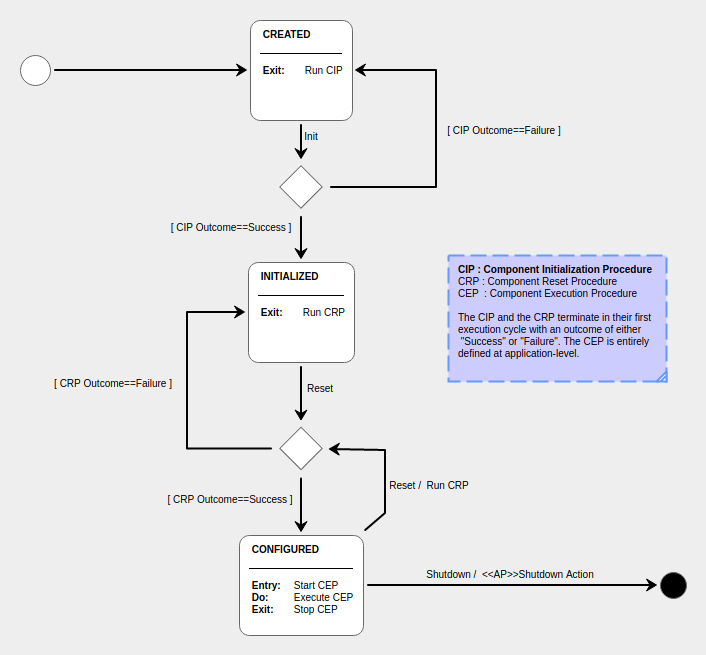
\includegraphics[scale=0.3,keepaspectratio=true]{BaseSM.png}
 \caption{Base State Machine}
 \label{fig:BaseSM}
\end{figure}

\begin{figure}[h]
 \centering
 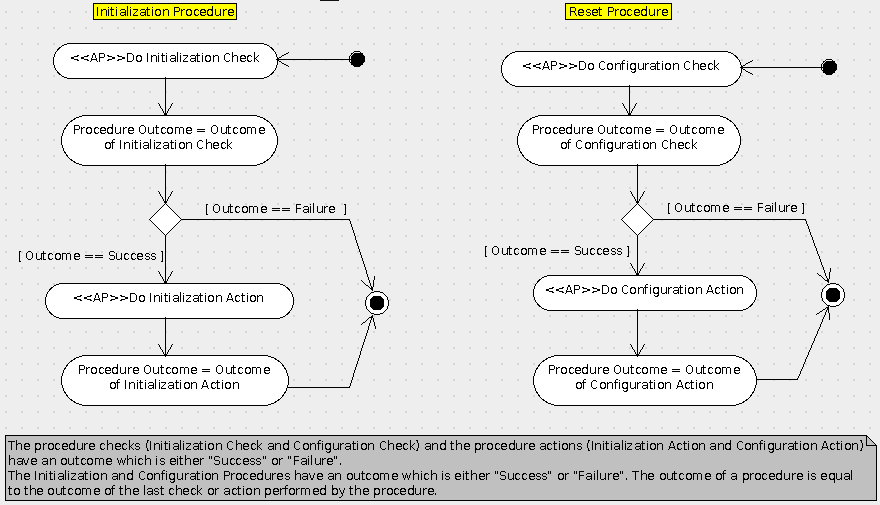
\includegraphics[scale=0.3,keepaspectratio=true]{InitializationAndReset.png}
 \caption{Initialization and Reset Procedures}
 \label{fig:InitializationAndReset}
\end{figure}

\begin{figure}[h]
 \centering
 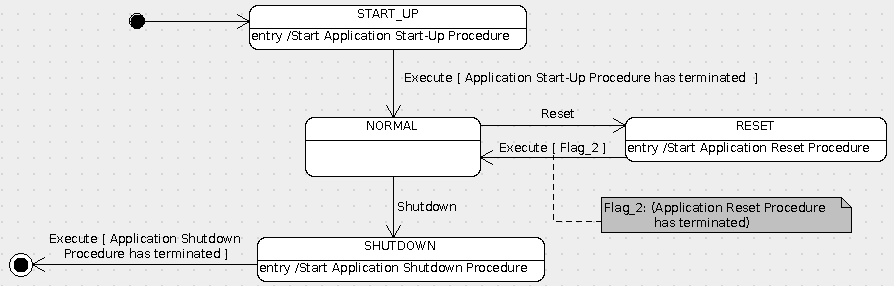
\includegraphics[scale=0.38,keepaspectratio=true]{ApplicationSM.png}
 \caption{Application State Machine}
 \label{fig:ApplicationSM}
\end{figure}

\begin{figure}[h]
 \centering
 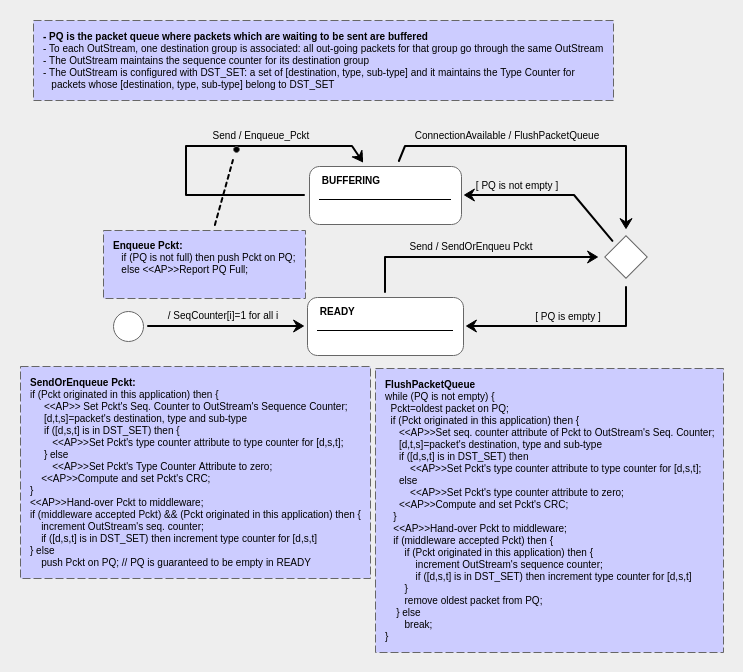
\includegraphics[scale=0.35,keepaspectratio=true]{OutStream.png}
 \caption{The OutStream State Machine}
 \label{fig:OutStream}
\end{figure}

\begin{figure}[h]
 \centering
 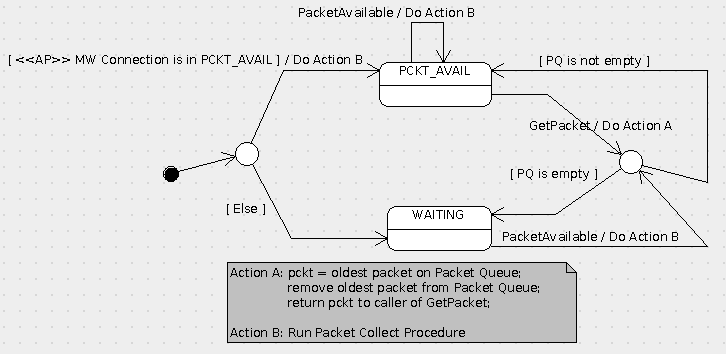
\includegraphics[scale=0.35,keepaspectratio=true]{InStream.png}
 \caption{The InStream State Machine}
 \label{fig:InStream}
\end{figure}

\begin{figure}[h]
 \centering
 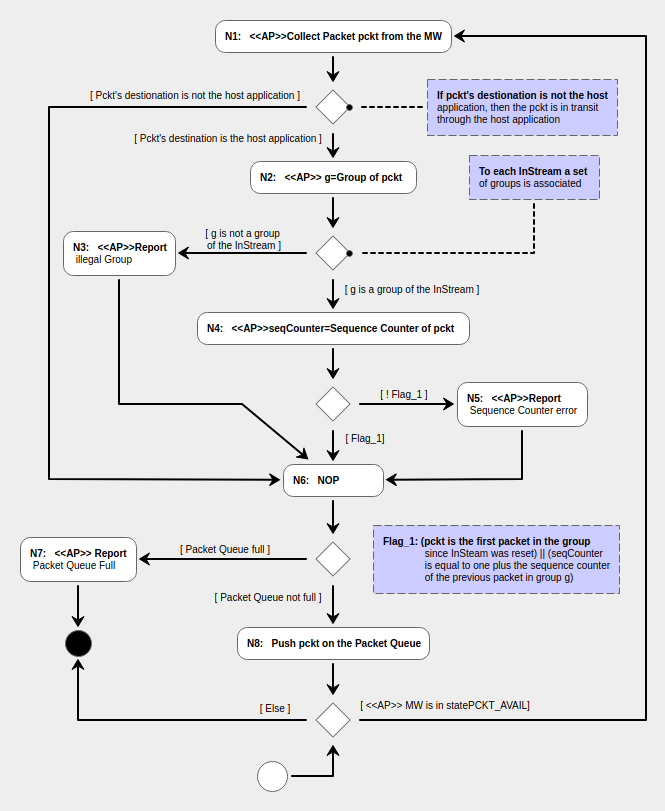
\includegraphics[scale=0.35,keepaspectratio=true]{PacketCollect.png}
 \caption{The Packet Collect Procedure}
 \label{fig:PacketCollect}
\end{figure}

\begin{figure}[h]
 \centering
 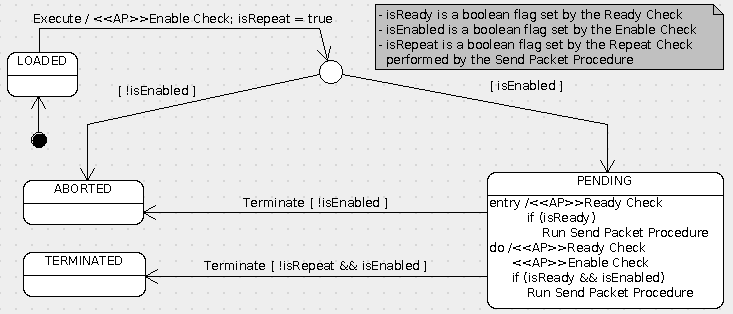
\includegraphics[scale=0.35,keepaspectratio=true]{OutComponent.png}
 \caption{The OutComponent State Machine}
 \label{fig:OutComponent}
\end{figure}

\begin{figure}[h]
 \centering
 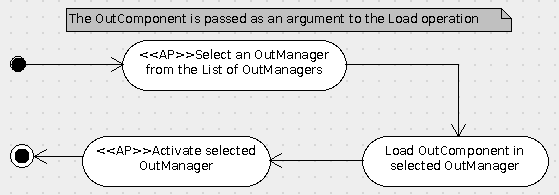
\includegraphics[scale=0.40,keepaspectratio=true]{OutLoaderLoad.png}
 \caption{The OutLoader Load Procedure}
 \label{fig:OutLoaderLoad}
\end{figure}

\begin{figure}[h]
 \centering
 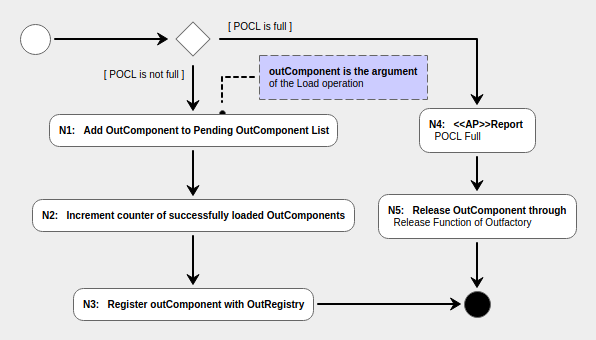
\includegraphics[scale=0.40,keepaspectratio=true]{OutManagerLoad.png}
 \caption{The OutManager Load Procedure}
 \label{fig:OutManagerLoad}
\end{figure}

\begin{figure}[h]
 \centering
 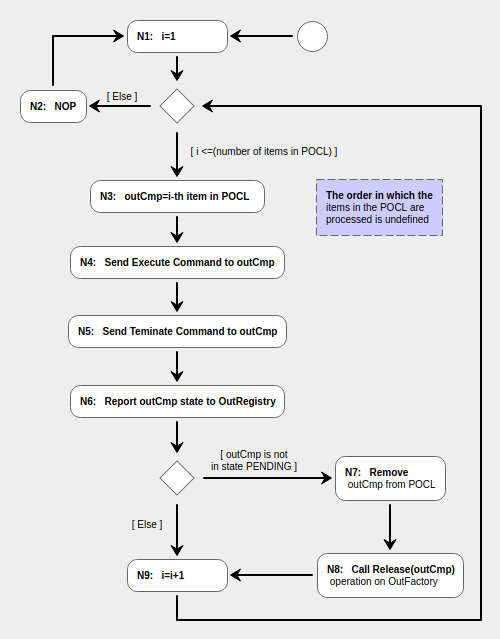
\includegraphics[scale=0.40,keepaspectratio=true]{OutManagerExecution.png}
 \caption{The OutManager Execution Procedure}
 \label{fig:OutManagerExecution}
\end{figure}

\begin{figure}[h]
 \centering
 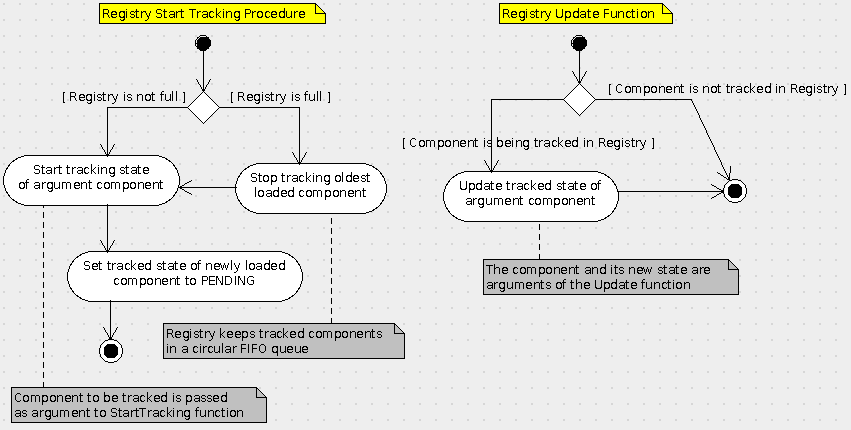
\includegraphics[scale=0.40,keepaspectratio=true]{RegistryStartTrackingAndUpdate.png}
 \caption{The Registry Start Tracking and Registry Update Procedures}
 \label{fig:RegistryStartTrackingAndUpdate}
\end{figure}

\begin{figure}[h]
 \centering
 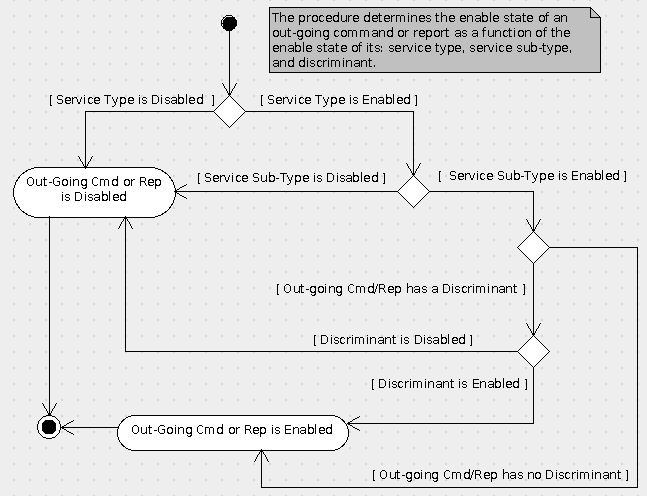
\includegraphics[scale=0.40,keepaspectratio=true]{EnableStateDetermination.png}
 \caption{The Enable State Determination Procedure}
 \label{fig:EnableStateDetermination}
\end{figure}

\begin{figure}[h]
 \centering
 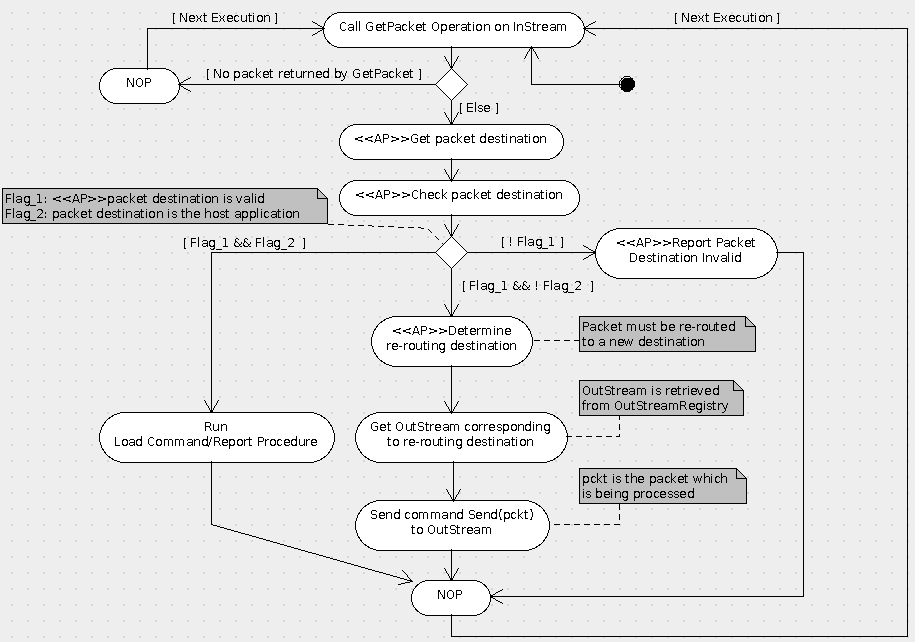
\includegraphics[scale=0.35,keepaspectratio=true]{InLoaderExecution.png}
 \caption{The InLoader Execution Procedure}
 \label{fig:InLoaderExecution}
\end{figure}

\begin{figure}[h]
 \centering
 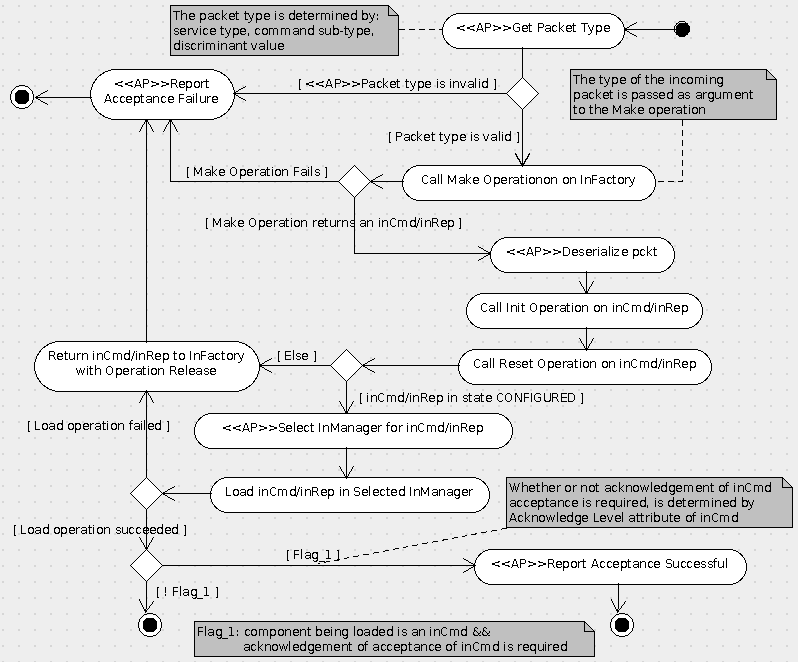
\includegraphics[scale=0.35,keepaspectratio=true]{InLoaderLoadCommandReport.png}
 \caption{The InLoader Load Command/Report Procedure}
 \label{fig:InLoaderLoadCommandReport}
\end{figure}

\begin{figure}[h]
 \centering
 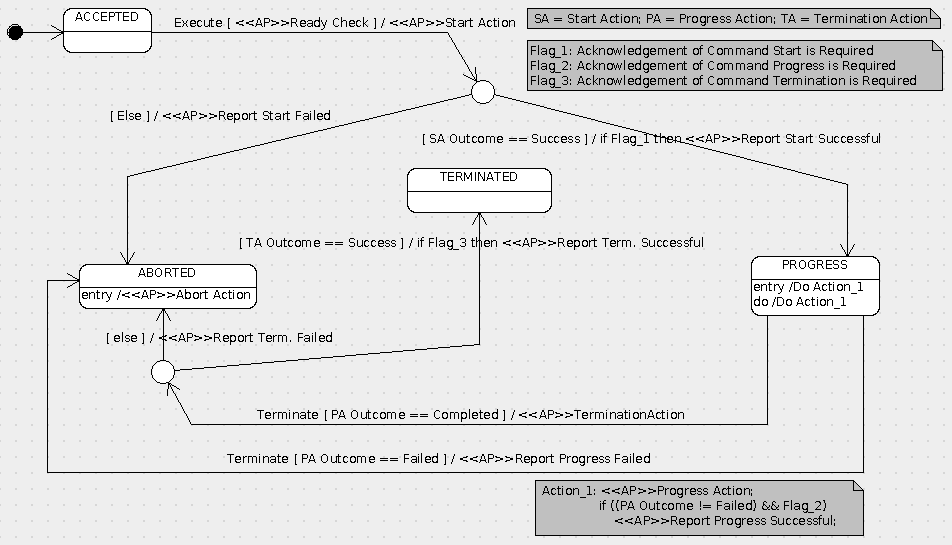
\includegraphics[scale=0.35,keepaspectratio=true]{InCommand.png}
 \caption{The InCommand State Machine}
 \label{fig:InCommand}
\end{figure}

\begin{figure}[h]
 \centering
 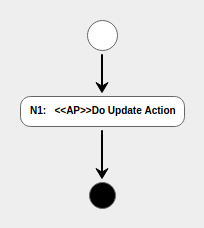
\includegraphics[scale=0.35,keepaspectratio=true]{InReportExecution.png}
 \caption{The InReport Execution Procedure}
 \label{fig:InReportExecution}
\end{figure}

\begin{figure}[h]
 \centering
 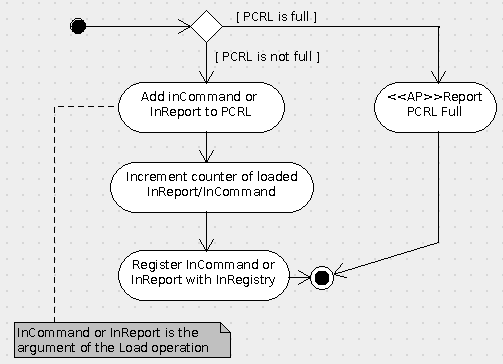
\includegraphics[scale=0.35,keepaspectratio=true]{InManagerLoad.png}
 \caption{The InManager Load Procedure}
 \label{fig:InManagerLoad}
\end{figure}

\begin{figure}[h]
 \centering
 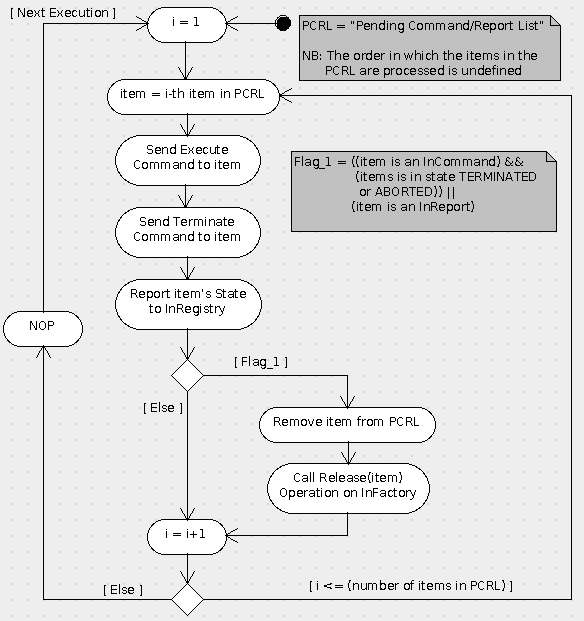
\includegraphics[scale=0.35,keepaspectratio=true]{InManagerExecution.png}
 \caption{The InManager Execution Procedure}
 \label{fig:InManagerExecution}
\end{figure}



%======================================================================================
\clearpage

\begin{thebibliography}{6}
 
\bibitem{ref:fwprofile} Alessandro Pasetti, Vaclav Cechticky:
           {\sl The FW Profile}. PP-DF-COR-00001, Revision 1.3,
           P\&P Software GmbH, Switzerland, 2013 

\bibitem{ref:C1Implementation} Alessandro Pasetti, Vaclav Cechticky:
           {\sl The Framework Profile - C1 Implementation User Manual}. 
           PP-UM-COR-00001, Revision 1.2.0,
           P\&P Software GmbH, Switzerland, 2013
		   Available from: \url{www.pnp-software.com/fwprofile}          
		   
\bibitem{ref:C1UserReq} Alessandro Pasetti, Vaclav Cechticky:
           {\sl The Framework Profile - C1 Implementation User Requirements}. 
           PP-SP-COR-00001, Revision 1.2.0,
           P\&P Software GmbH, Switzerland, 2013
		   Available from: \url{www.pnp-software.com/fwprofile}          		     
           
\bibitem{ref:cordetfw} Alessandro Pasetti, Vaclav Cechticky:
           {\sl The CORDET Framework}. 
           PP-DF-COR-00002, Revision 1.3.0,
           P\&P Software GmbH, Switzerland, 2014   
           
\bibitem{ref:C2Implementation} Alessandro Pasetti, Vaclav Cechticky:
           {\sl The CORDET Framework - User Manual}. 
           PP-UM-COR-00002, Revision 0.4.0,
           P\&P Software GmbH, Switzerland, 2014                  
           
\end{thebibliography}

\end{document}          

